% Edit this section directly. Styling is in raylo-report.sty.
\section{How many categories is the right number}
Stakeholders asked whether 275 was too many, too few, or arbitrary. We tested both directions, and the answer turned out to depend on the model that consumes the categories, so it is given in two parts.

Collapsing, with the simple August model: the same features were rebuilt at seven levels of detail from 275 leaves down to 4 broad groups, and the August XGBoost trained at each, three seeds with bootstrap intervals. The 275-leaf, 69-group and 29-group views were statistically indistinguishable. Seventeen groups was close but showed a small, real loss on the six-month outcome. Nine and fewer degraded clearly. The 69-group view is worth explaining because it causes confusion: it is today's model-feature grouping, in which 40 leaves each get their own feature block and the other 235 are rolled into their 29 general categories. All 275 leaves are still classified; none are dropped.

Collapsing, with the champion recipe of section 10: the same ladder was re-run with the stronger recipe and its richer per-category features once that became the reference model. Given every column, the six-month outcome now rewards detail: 275 leaves scores 0.612 against 0.586 for today's 69 groups, falling steadily to 0.510 at 4 groups. The three-month outcome does not; its peak is the 69-group view and 275 sits marginally below it. Under a hard 50-feature cap the picture inverts. The 275-leaf rung becomes the worst on both outcomes, because roughly 2,900 thin per-leaf candidates crowd the handful of broad, information-dense features (priority-debt breadth, months with credit products) out of the 50 slots: only 2 of those 31 spine columns survive selection at 275 leaves, against 9 at 17 groups. That is a property of feature selection from a very wide pool, not of the taxonomy, and it is why the capped champion in section 10 selects from a base that keeps those spine features rather than from the raw leaf pool.

Expanding: three well-supported parents (streaming, general marketplace, payment intermediary) were split into 15 shadow children, a simulated move from 275 to 287 leaves, with the rules frozen before any outcome was inspected. Against a control that received the exact parent totals, the split features changed GINI by between minus 0.002 and minus 0.011, with every confidence interval including zero. Payment intermediary on its own produced a small but clear loss. This was not a thin-data result: the shadow categories appeared in 54,000 of 64,000 modelling rows.

\begin{figure}[H]
\centering
\ChartTitle{Figure 1. Risk-model GINI by number of category groups, August recipe (same cohort, same learner, 3 seeds)}
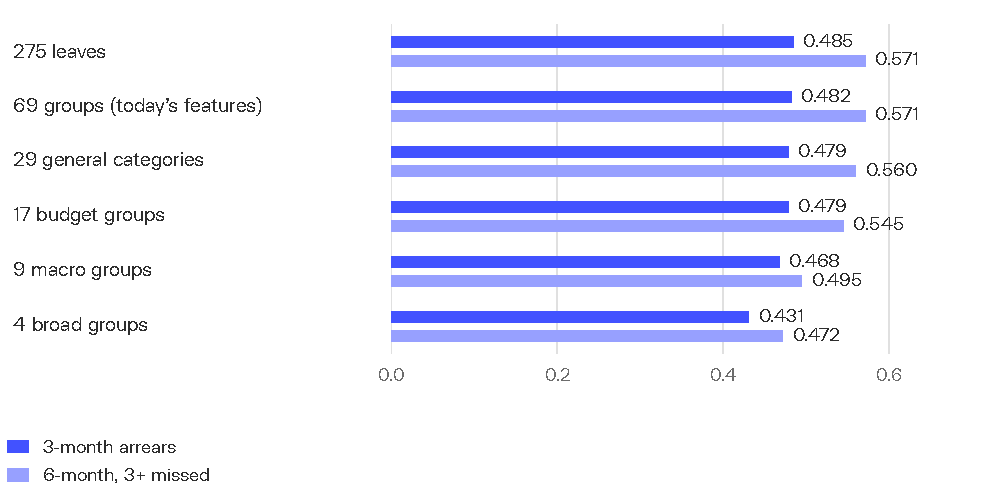
\includegraphics[width=\linewidth]{charts/fig-ladder.pdf}
\caption*{August recipe: a single XGBoost on rung-level counts and amounts, uncapped, 3 seeds. Collapsing the 275 leaves to 69 or 29 groups costs nothing measurable; 17 begins to lose the six-month signal; 9 and fewer degrade clearly. Predates the September as-of rebuild; directional.}
\end{figure}
\begin{figure}[H]
\centering
\ChartTitle{Figure 2. The same ladder with the champion recipe, six-month GINI, single XGBoost}
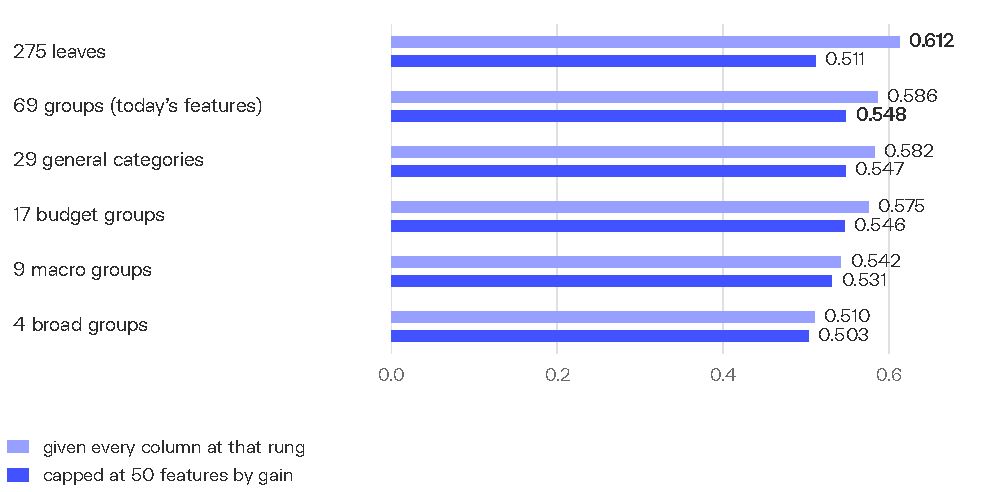
\includegraphics[width=\linewidth]{charts/fig-ladder-champ.pdf}
\caption*{Champion recipe with its richer per-category features, rebuilt at each rung on a recipe-neutral base so only granularity changes. Given every column, finer is better on the six-month outcome. Capped at 50, the 275-leaf rung is worst because its 2,900 thin candidates crowd the strongest broad features out of the selection. The three-month outcome shows no gain from detail in either setting; 69 groups is its peak.}
\end{figure}
\subsection{Reconciling the two results}
The two ladders look contradictory and are not. They answer different questions, and the same three facts hold across both.

\begin{enumerate}
\item \textbf{Whether detail helps depends on what the model can do with it.} The August model built one count and one amount per category. At that level of description, 275 leaves carried no more usable signal than 29 groups, because most of what a leaf adds over its parent is in how the spending is distributed, not in its total. The champion builds per-leaf shares and averages, and with those in hand the six-month model finds real signal in the fine leaves. The three-month horizon is noisier and shorter, and does not, under either recipe.
\item \textbf{A hard feature cap is a selection problem, not a taxonomy problem.} Ranking 2,900 candidate columns by gain and keeping 50 is unreliable: thin per-leaf columns outnumber the handful of broad, strong features by a hundred to one, and the strong ones are squeezed out. That is why the 275-leaf rung scores worst when capped from the raw pool. The capped champion in section 10 avoids this by selecting from a base that already contains the broad features alongside the leaf-level ones, and reaches 0.588 where the raw-pool rung reaches 0.511.
\item \textbf{The taxonomy decision is the same under every reading.} Categories are stored at 275 leaves because a leaf can always be rolled up at feature-build time and a rollup can never be split back. Which rollup or feature pool a given model consumes is a modelling choice, made per model and per outcome, and validated the way the capped champion was.
\end{enumerate}
\begin{tcolorbox}[colback=BlueTint,colframe=Blue,boxrule=0pt,leftrule=2pt,arc=3mm]
Keep 275 leaves as the governed source of truth. Detail is reversible, since a leaf can be rolled up at feature-build time, while deletion is not, and the stronger the model, the more the six-month outcome rewards that detail. Let each model consume a validated rollup or a curated feature pool, and keep proposed new categories in shadow until they show stable value.
\end{tcolorbox}
